% THIS TEMPLATE IS A WORK IN PROGRESS
% Adapted from an original template by faculty at Reykjavik University, Iceland

\documentclass{scrartcl}

% Adapted from an original template by Hlyni Arnórssyni, Reykjavik University, Iceland
%
% ------------------------------ SETTINGS
\usepackage{geometry}

\geometry{
	paper=a4paper, % Paper size
	top=2.5cm, % Top margin
	bottom=2.5cm, % Bottom margin
	left=2.5cm, % Left margin
	right=2.4cm, % Right margin
	headheight=0.75cm, % Header height
	footskip=1.5cm, % Space from the bottom margin to the baseline of the footer
	headsep=0.75cm, % Space from the top margin to the baseline of the header
	%showframe, % Uncomment to show how the type block is set on the page
}

\usepackage{blindtext}
%-------------------------------- Character encoding ----------------------------
\usepackage[T1]{fontenc}
\usepackage[utf8]{inputenc}

%----------------------------- Mathematics packages from AMS ---------------

\usepackage{amsmath, amsfonts, amsthm, amssymb}
\usepackage{braket, nicefrac}

% ----------- International System of Units
\usepackage{siunitx}

%------------------------------ Lists / numbers -------------------------
\usepackage{enumitem, multicol}

%------------------------------- Figure insertions --------------
\usepackage{graphicx, float}  % Use option [H] to force the placement of a figure
\usepackage{keystroke}
\usepackage{pgfplots}\usepgfplotslibrary{units}\pgfplotsset{compat=1.16}

%------------------------------- Line Spacing --------------
\usepackage{setspace}

%------------------------------- Depth of the ToC --------------
\setcounter{tocdepth}{2}

%%%%%%%%%%%%%%%%%%%%%%%%%% Hyperlink References %%%%%%%%%%%%%%%%%%%%%%%%%%%
\usepackage{hyperref}

%--------------------% Storage Path for images %-----------------%
\graphicspath{{graphics/}{Graphics/}{./}{./research-paper/capstone/capstone/Graphics}}

%%%%%%%%%%%%%%%%%%%%%%%%%% Environments %%%%%%%%%%%%%%%%%%%%%%%%%%%
\renewenvironment{abstract}{
    \begin{center}
    \textbf{Abstract}
    \vspace{0.5cm}
    \par\itshape
    \begin{minipage}{0.8\linewidth}}{\end{minipage}
    \noindent\ignorespaces
    \end{center}
}

\newenvironment{keywords}{
    \begin{center}
    \textbf{Keywords}
    \vspace{0.5cm}
    \par
    \begin{minipage}{0.8\linewidth}}{\end{minipage}
    \noindent\ignorespaces
    \end{center}
}

\newenvironment{preface}{
    \begin{center}
    \textbf{Preface}
    \vspace{0.5cm}
    \par
    \begin{minipage}{0.8\linewidth}}{\end{minipage}
    \noindent\ignorespaces
    \end{center}
}

\newenvironment{acknowledgements}{
    \begin{center}
    \textbf{Acknowledgements}
    \vspace{0.5cm}
    \par
    \begin{minipage}{0.8\linewidth}}{\end{minipage}
    \noindent\ignorespaces
    \end{center}
}

\hbadness=10000

\begin{document}
%Title of the report, name of coworkers and dates (of experiment and of report).
\begin{titlepage}
	\centering
	
\includegraphics[width=0.6\textwidth]{nyush-logo.jpeg}\par
	\vspace{2cm}
	%%%% COMMENT OUT irrelevant lines among the 3 below
	{\scshape\LARGE Computer Science, Data Science \& \par}  %if you're a CS major
	{\scshape\LARGE Computer Systems Engineering \par}
	\vspace{1cm}
	{\scshape\Large Capstone Report - Fall 2024\par}
	%{\large \today\par}
	\vfill

	%%%% PROJECT TITLE
	{\huge\bfseries Benchmarking ZK Virtual Machines for Privacy-Preserving Machine Learning Applications\par}
	\vfill

	%%%% AUTHOR(S)
	{\Large\itshape Lawrence Lim\\ Siddhartha Tuladhar\\ Brandon Gao\\}\par
	\vspace{1.5cm}

	\vfill
	supervised by\par
	%%%% SUPERVISOR(S)
	Promethee Spathis

	\vfill
	% Bottom of the page
\end{titlepage}

\newpage

\begin{preface}
	As a team comprising a Computer Systems Engineering major, a Computer Science major, and a Data Science major, we bring diverse perspectives and expertise to address the complex challenges at the intersection of privacy, security, and scalability in technology. This project was inspired by the increasing importance of privacy-preserving computation, particularly in sensitive fields like finance, where secure data handling is paramount. Our collective academic backgrounds have allowed us to explore innovative approaches to these challenges, drawing from distributed systems, cryptography, and data analytics.

	Our target audience includes researchers, developers, and industry professionals who are advancing privacy technologies, blockchain systems, and secure data frameworks. By benchmarking zero-knowledge virtual machines (zkVMs) in the context of financial data, this project seeks to provide valuable insights into their capabilities and limitations, contributing to the ongoing development of secure and privacy-centric computational tools.
\end{preface}

\vspace{1cm}

\begin{acknowledgements}
	We sincerely thank our advisor, Professor Promethee Spathis, for their guidance and support throughout this project. We are also grateful to the Professor Benedikt Bunz for providing the initial ideation for this project. Lastly, we are grateful to our families and friends for their encouragement and support.\end{acknowledgements}

\newpage

\begin{abstract}
	This work addresses the challenge of securely processing sensitive data in privacy-critical applications like finance. Zero-knowledge virtual machines (zkVMs) offer a promising solution, but face issues with complexity and proof generation time. We benchmark three zkVMs—SP1, Jolt, and RISC-0—by training a ridge regression model on financial data, evaluating their performance and identifying key bottlenecks. Our findings highlight zkVMs’ potential for privacy-preserving computation and provide insights for improving their practical adoption.
\end{abstract}
\vspace{1cm}

\begin{keywords}
	\centering
	\textbf{Capstone; Computer science; Machine Learning; Zero-Knowledge Proofs, Zero-Knowledge Virtual Machines, Jolt, SP1, Risc0, NYU Shanghai}
\end{keywords}

\newpage



\doublespacing
\tableofcontents
\singlespacing

\newpage

\doublespacing

\section{Introduction}

\subsection{Context}

Currently, there exists a large amount of sensitive customer data that is extremely valuable but not being monetized to its fullest extent due to a combination of compliance and ethical concerns. An essential category of this data is personal financial data. Due to the sensitive nature of this data and strict compliance laws, current Fintech platforms require users’ explicit permission to access sensitive information like credit history, transaction history, and income. However, \textbf{Zero Knowledge Proof (ZKP)} can be utilized to develop services and algorithms that utilize the sensitive data without explicitly revealing it. A ZKP is a cryptographic method of proving a statement is true without revealing any other information besides the fact that the statement is true. ZKPs have three fundamental characteristics:

\begin{itemize}
	\item \textbf{Completeness:} If a statement is true, an honest prover can prove to an honest verifier that they have knowledge of the correct input.
	\item \textbf{Soundness:} If a statement is false, a dishonest prover is unable to convince an honest verifier that they have knowledge of the correct input.
	\item \textbf{Zero-knowledge:} No other information about the input is revealed to the verifier from the prover besides the fact that the statement is true.
\end{itemize}

Currently, the most-friendly way of generating a ZKP is through the use of zero-knowledge virtual machines (zkVMs). A zkVM, is simply a VM implemented as a circuit for a ZKP system. So, instead of proving the execution of a program, as one would normally do in ZKP systems, you prove the execution of the bytecode of a given Instruction Set Architecture (ISA). However, the zkVM landscape is in early development, and proof generation is bottlenecked by the complexity of the program and hardware limitations. In this paper, we provide a quantatitve and qualitative analysis on the current state of zkVMs on a real-world use case by generating a proof of a machine learning (ML) algorithm on dummy financial data.

\subsection{Objective}

The objective of this paper is to provide researchers, developers, and industry professionals a comprehensive comparable analysis of zkVMs in real-world use cases. To achieve this, we benchmark SP1\cite{Roy2024}, Risc0\cite{bruestle2023risc}, and Jolt\cite{arun2024jolt}. They all compile to RISC-V, which is an extremely popular compile target for common programming languages (Rust, C++, LLVM). We provide a quantative analysis on proof generation time and proof verification time. Additionally, we provide a qualitative analysis on the zkVM developer experience and how their performance trade-offs can impact real-world applications.

\section{Related Work}

%%%% DO NOT write a related work section that is just a laundry list of other papers, with a sentence about each one that was lifted from its abstract, and without any critical analysis nor deep comparison to other work.

\subsection{Zero Knowledge Virtual Machines}

Our research compares the most efficient methods for generating ZKPs for machine learning algorithms by experimenting with different zkVMs. The current papers on zkVMs focus on their architecture and the techniques that are used by the zkVM to achieve optimized proof and verification times. The first zkVM was presented by Bruestle and Gafni\cite{bruestle2023risc}, who introduced RISC-0, a system designed to produce scalable, transparent proofs for computations based on the RISC-V instruction set. RISC-0 also optimized heavily for proof performance on GPUs. Following RISC-0's success, Uma Roy\cite{Roy2024} introduced SP1, a performant zkVM similar to RISC-0, but with slight modifications to the SNARK proof system and the extensive use of hand optimized precompiles that make certain operations (hash functions, signatures, elliptic curve arithmetic, etc.) quicker to prove within the zkVM. It's worth noting, that SP1 does not have a paper. In mid 2024, Arun et al.\cite{arun2024jolt} presented Jolt, a zero-knowledge Succinct Non-Interactive Argument of Knowledge (zkSNARK) system optimized for VMs, which uses a new lookup technique that makes Jolt faster at generating proofs while maintaining a quick verification time.

\subsection{Machine Learning in ZKPs}

Machine learning is a highly relevant use case for ZKPs. There are multiple papers on the various use cases of ML in ZKPs. Wang et al.\cite{wang2024efficient} developed an efficient ZKP-based pipeline for classical machine learning inference, focusing on privacy-preserving inference that ensures model accuracy without exposing sensitive model information. Their system optimizes zero-knowledge inference, making it highly applicable to real-world ML applications where data privacy is paramount. Our work also uses inference in a similar within the zkVM as a real world application. Similarly, Sathe et al.\cite{sathe2024survey} provide a comprehensive survey of ZKP applications in machine learning, covering a range of cryptographic techniques and their applicability to neural networks, decision trees, and other ML models. Their survey offers a broader comparison of ZKP techniques in the ML space, providing essential context for more specific systems like that of Wang et al. However, their paper does not provide details on the performance or real-world use case. Lastly, Ganescu and Passerat-Palmbach\cite{ganescu2024trust} extend the application of ZKPs to generative AI models, by proposing a system that enhances trust in AI by allowing for the verification of generative models without exposing underlying data, which is critical in AI-driven environments where sensitive inputs and outputs must be safeguarded while still proving the model’s validity. This paper is similar to Wang et al., where it provides a real-world use case, but it focuses on hand-written ZK circuits which requires a high degree of zero-knowledge cryptography experience to write. This is inaccessible to developers and requires orders of magnitude more high development overhead compared to convensional programming techniques. By using zkVMs, most of the ZKP logic is abstracted away, allowing developers to focus on the application itself and privacy-preserving logic (if applicable).

\section{Solution}

The methodology for achieving our objective is structured into two key phases. The first phase involves developing and training a machine learning algorithm on a given dataset to attain satisfactory accuracy levels. The second phase required us to export the trained model and test data into Rust, where the inference process is implemented by manually translating the logic from Python to Rust. Finally, we set different test input sizes and benchmarked the proving and verification of the algorithm in the three zkVMs and on different machines.

\subsection{Machine Learning Setup}

In order to simulate real-world transaction data, historical transaction data was taken from a Kaggle dataset\cite{rehman2023retail}. The dataset comprised of customer transactions, with each record containing information on the transaction date, product price, quantity purchased, and customer ID. The first step in the data preparation process involved determining a cutoff date that would separate the historical data used for training from the future data we wish to predict. We defined this cutoff date as 90 days before the latest transaction in the dataset. This allowed us to segment the data into two parts:

\begin{itemize}
	\item \textbf{Training Data (First Three Quarters):} Transactions occurring before the cutoff date, which we used to derive customer behavior features (recency, frequency, and monetary values).
	\item \textbf{Target Data (Fourth Quarter):} Transactions occurring after the cutoff date, which were used to calculate the target variable, customer spending in the last quarter (\texttt{actual\_spend\_90\_days}).
\end{itemize}

We aimed to predict customer spending for the next 90-day period (i.e., the last quarter) based on historical transaction data. We used these defined fiscal quarters to organize the data, aggregating customer spending within each quarter to track how spending evolves over time. The ultimate goal was to use the data from Q1, Q2, and Q3 to predict customer spending in Q4.

Next, the dataset was processed to extract key features such as recency, frequency, monetary value (RFM), and spending activity, which is depicted in Table \ref{tab:dataset_description}. RFM serves as a foundation for predictive modeling, where these metrics can be combined with other features to enhance the accuracy of customer spending predictions.

\begin{table}[ht!]
	\centering
	\begin{tabular}{|l|p{10cm}|}
		\hline
		\textbf{Field}                   & \textbf{Description}                                                                          \\
		\hline
		\textbf{CustomerID}              & Unique identifier for a customer, used to track and differentiate individuals in the dataset. \\
		\hline
		\textbf{Frequency}               & Number of transactions a customer made during the first three quarters.                       \\
		\hline
		\textbf{Monetary}                & Total monetary value of a customer's transactions during the first three quarters.            \\
		\hline
		\textbf{Recency}                 & Number of days since the customer's last transaction during the first three quarters.         \\
		\hline
		\textbf{Price}                   & Price per unit for each transaction item.                                                     \\
		\hline
		\textbf{DiscountApplied}         & Percentage of discount applied to the transaction.                                            \\
		\hline
		\textbf{spend\_90\_flag}         & Binary flag indicating whether the customer made any transaction in the past 90 days.         \\
		\hline
		\textbf{actual\_spend\_90\_days} & Total amount spent by the customer in the last 90 days(quarter).                              \\
		\hline
	\end{tabular}
	\caption{Description of fields in the customer transaction dataset.}
	\label{tab:dataset_description}
\end{table}

For the machine learning algorithm, we used the Ridge Regression Model due to the model's accuracy and the complexity constraints of the zkVMs. Ridge Regression is an extension of linear regression by adding a penalty term to the loss function to prevent overfitting.  Ridge Regression prevents overfitting by penalizing large coefficient values, thereby shrinking them towards zero. The Ridge Regression loss function is formulated as:
\[
	\text{Loss} = \sum_{i=1}^{m} \left( y_i - \hat{y}_i \right)^2 + \lambda \sum_{j=1}^{n} w_j^2
\]
where \( m \) is the number of samples, \( n \) is the number of features, \( \hat{y}_i \) represents the predicted value for the \( i \)-th sample, \( \lambda \) is the regularization parameter controlling the strength of the penalty, and \( w_j \) are the model coefficients. The second term \( \lambda \sum_{j=1}^{n} w_j^2 \) is the regularization term, which discourages large coefficients and helps reduce the model's variance. The accuracy of the model is shown in Table \ref{tab:model-performance}.

\begin{table}[!ht]
	\centering
	\begin{tabular}{|l|c|p{8cm}|}
		\hline
		\textbf{Metric}         & \textbf{Value} \\
		\hline
		\( R^2 \)(R-Squared)    & 0.8            \\
		\hline
		Mean Square Error (MSE) & 21             \\
		\hline
	\end{tabular}
	\caption{Model performance metrics.}
	\label{tab:model-performance}
\end{table}

The \(R^2\) value measures the proportion of variance in the target variable that is explained by the independent variables in the model. It ranges from 0 to 1, where higher values indicate a better fit of the model to the data. The \(R^2\) value of 0.8 demonstrates that the model explains a substantial portion of the variance in the target variable, effectively capturing the relationships in the data.

The MSE represents the average squared difference between the predicted and actual values. It provides a measure of the model's prediction error, with lower values indicating better performance. The MSE value of 21 is acceptable because it aligns well with the scale of the target variable.

\subsection{zkVM Implementation}

Figure \ref{fig:architecture} illustrates the high-level architecture of the zkVM implementation. In this framework, the ML model and inference data serve as inputs to each of the three zkVMs. Using the provided ML model, the zkVMs predict a specific customer’s transaction amount and generate a ZKP that ensures the integrity of the inputs and outputs. Users can access the output by referencing the corresponding ZKP object. To validate the correctness of the output, each zkVM incorporates a verification function that enables users to confirm whether the output was accurately derived from the ML algorithm.

\begin{figure}[H]
	\begin{center}
		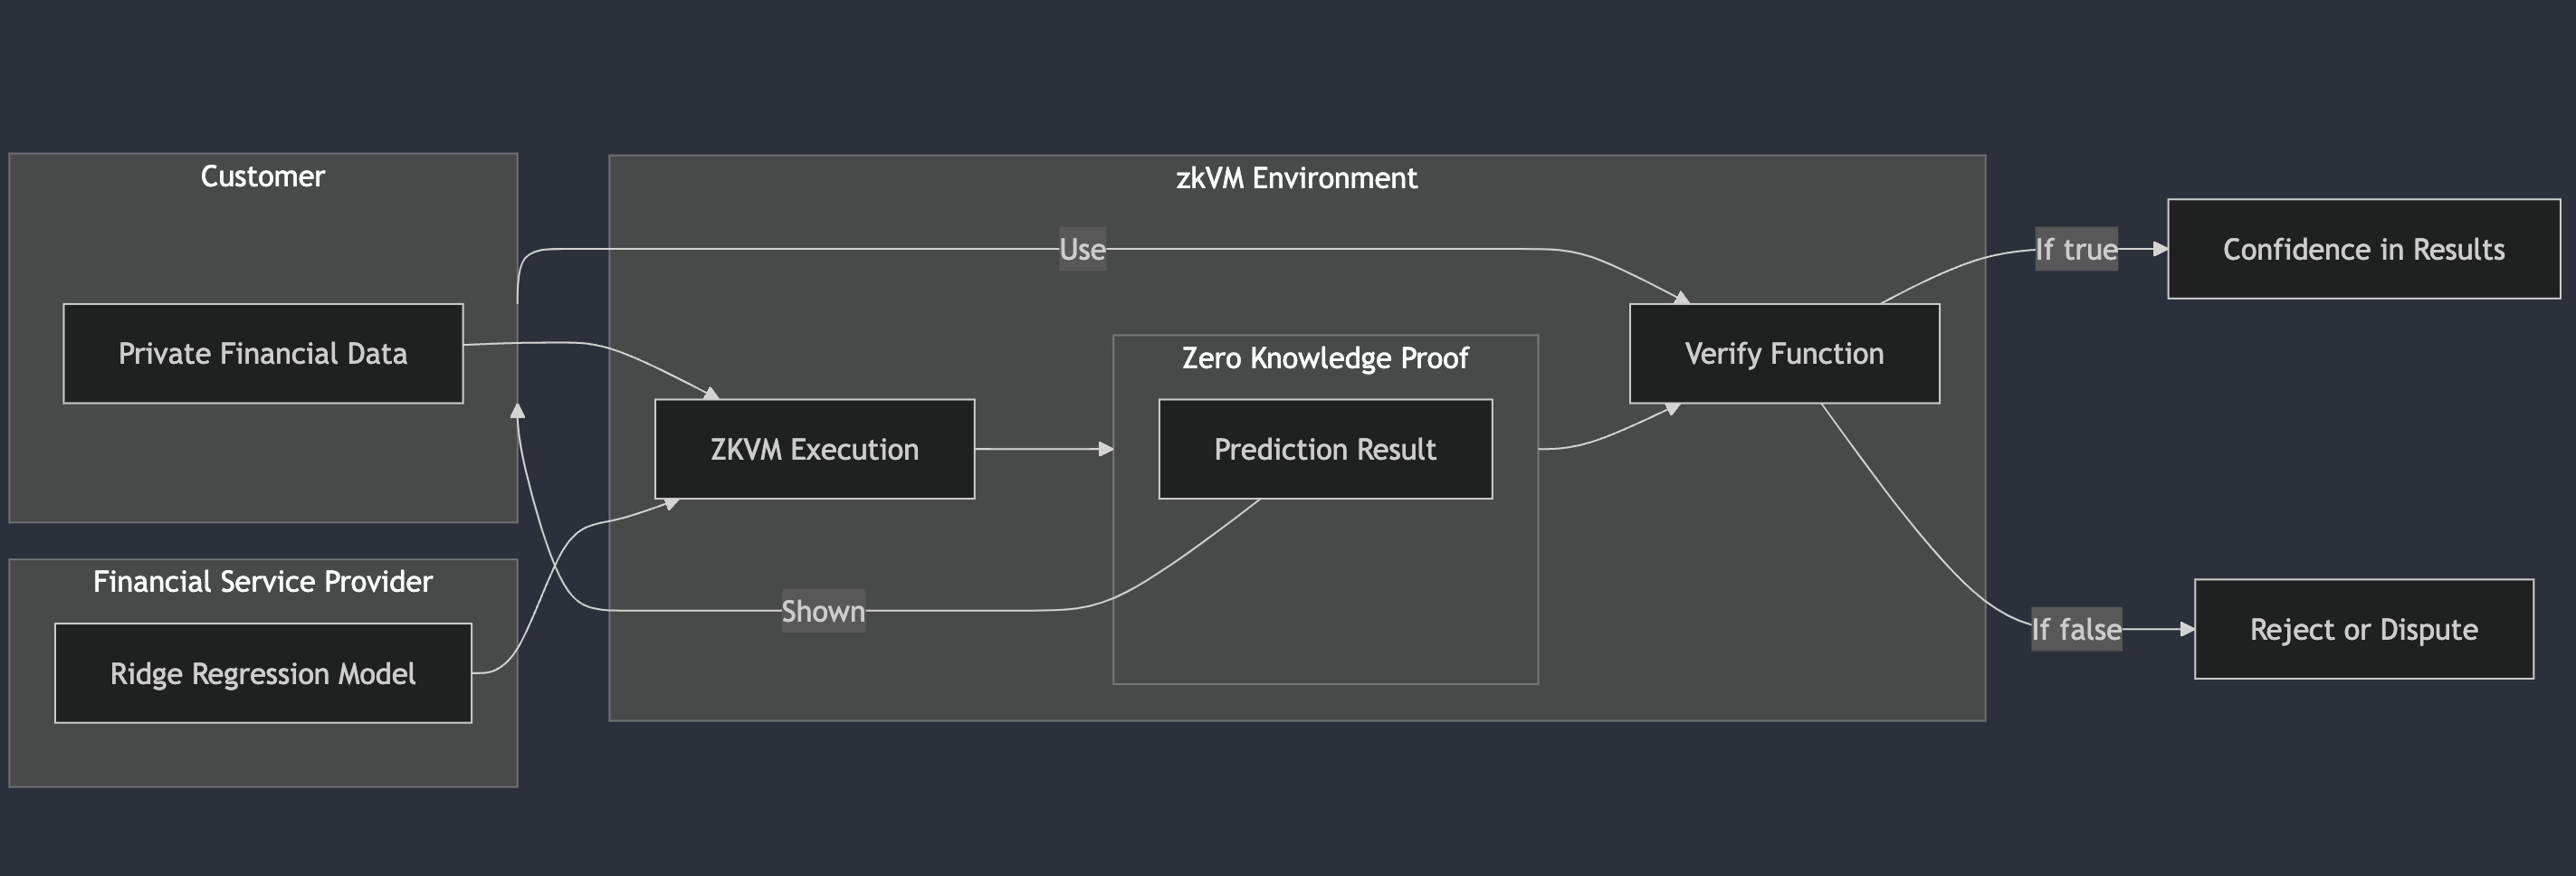
\includegraphics[scale=0.35]{zkVM-design.png}
	\end{center}
	\caption{Architecture of our benchmark procedure}
	\label{fig:architecture}
\end{figure}

The benchmarking process for all three zkVMs involved measuring the time required for proof generation and verification. Timing was recorded by initiating a timer at the start and end of each process. This evaluation was conducted across varying numbers of inference test cases and was performed on both ARM-based and x86-based computing platforms to compare performance across architectures.

\section{Results}

\subsection{Quantatitve Results}

The results section details your metrics and experiments for the assessment of your solution. It then provides experimental validation for your approach with visual aids such as data tables and graphs. In particular, it allows you to compare your idea with other approaches you've tested, for example solutions you've mentioned in your related work section.

The results are categorized based on the architecture of the machines utilized to run the zkVMs.

\subsubsection{ARM Benchmark}

\begin{figure}
	\begin{center}
		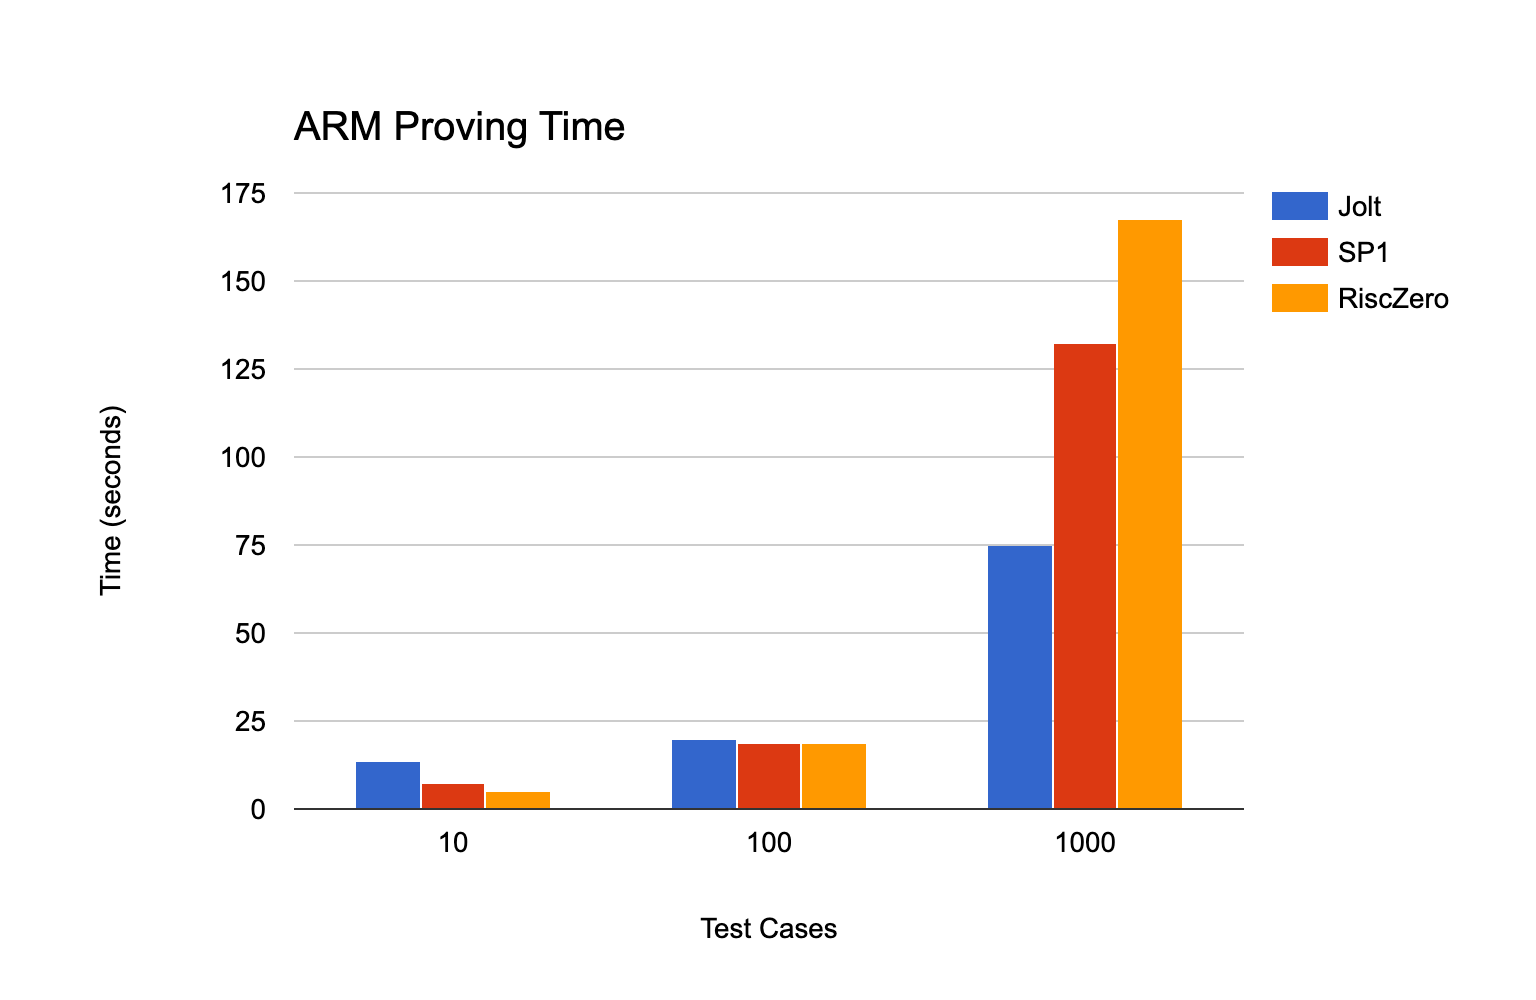
\includegraphics[width=\linewidth]{ARM-Proving-Time.png}
	\end{center}
	\caption{Proof Generation Benchmark for Jolt, SP1, and RISC-0 on ARM chip}
	\label{graph:arm-proving-time}
\end{figure}

The ARM benchmarks were conducted on an M1 Max Apple Mini, a RISC-based system equipped with 10 CPU cores and 64GB of RAM. Figure \ref{graph:arm-proving-time} presents a comparative analysis of the time required to generate the ML proof. The results indicate that SP1 was the fastest for 10 test cases, completing the proof generation in 7.46 seconds. For 1000 test cases, Jolt demonstrated the best performance, achieving proof generation in 15.10 seconds. Conversely, Jolt exhibited the longest runtime for 10 test cases at 13.57 seconds, while Risc0 recorded the slowest performance for 1000 test cases, taking 132.13 seconds to generate the proof.

\begin{figure}
	\begin{center}
		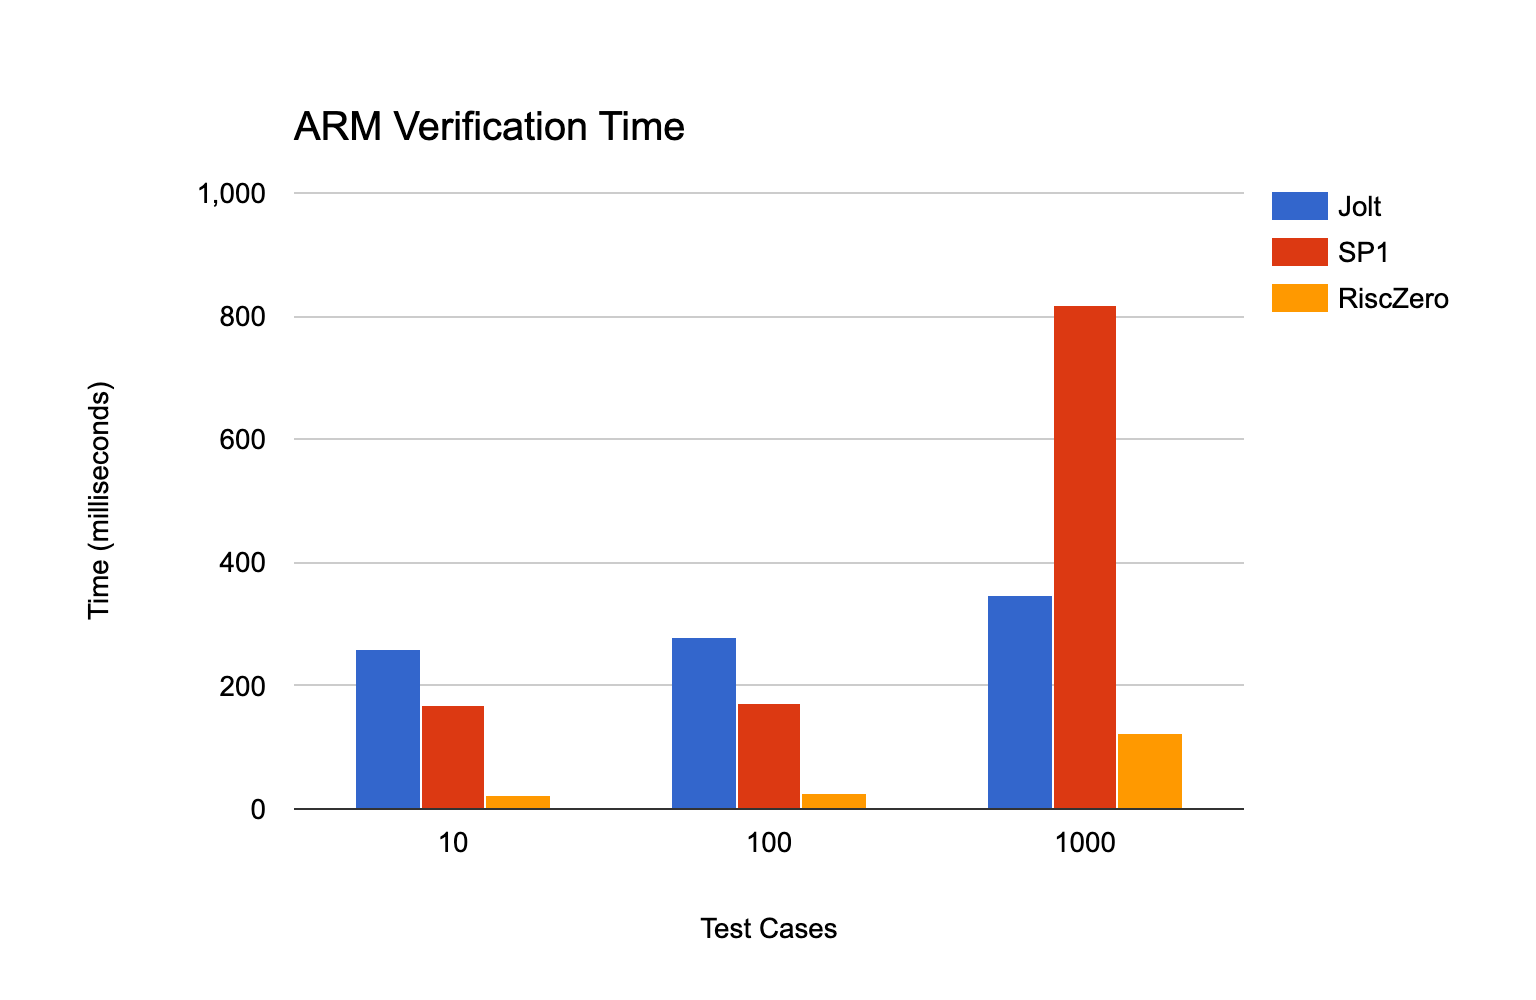
\includegraphics[width=\linewidth]{ARM-Verification-Time.png}
	\end{center}
	\caption{Proof Verification Benchmark for Jolt, SP1, and RISC-0 on ARM chip}
	\label{graph:arm-verification-time}
\end{figure}

Proof generation is typically efficient, and due to the property of succinctness inherent in ZKPs, verification in theory is expected to operate in  O(1) time complexity. Figure \ref{graph:arm-verification-time} showcases the proof verification benchmark on ARM architecture. The slowest performance for 10 test cases was observed with Jolt, taking 259.08 ms, while Risc0 achieved the fastest verification time at 22.73 ms. At 1000 test cases, Risc0 maintained its superior performance with a verification time of 124.53 ms, whereas SP1 exhibited the slowest verification time, significantly lagging at 818.74 ms.

\subsection{x86 Benchmark}

The x86 benchmarks were performed on an Intel Cascade Lake Platinum 8268 processor, a CISC-based architecture featuring 18 CPU cores and 180GB of RAM. Figure \ref{graph:x86-proving-time} illustrates a comparison of the time required to generate machine learning proofs on the x86 architecture. At 10 test cases, proof generation was the slowest on Jolt, taking 13.62 seconds, while Risc0 demonstrated the fastest performance at 9.62 seconds. For 1000 test cases, Jolt exhibited significantly improved performance, completing proof generation in 69.36 seconds, whereas Risc0 required 309.14 seconds, making it over four times slower.

\begin{figure}
	\begin{center}
		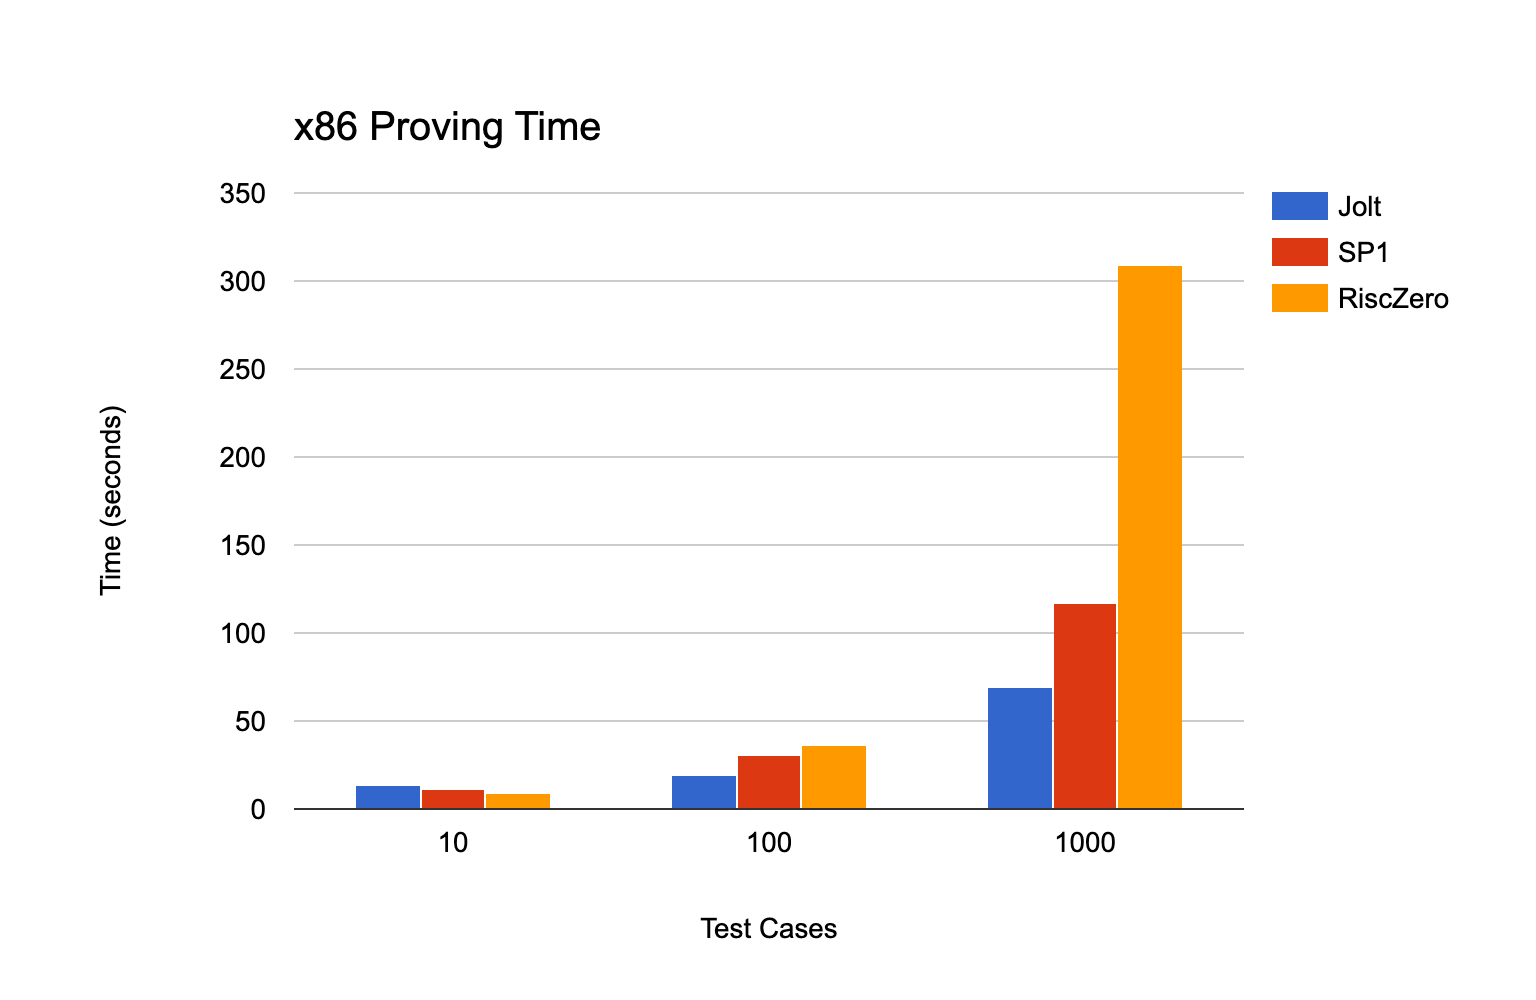
\includegraphics[width=\linewidth]{x86-Proving-Time.png}
	\end{center}
	\caption{Proof Generation Benchmark for Jolt, SP1, and RISC-0 on x86 chip}
	\label{graph:x86-proving-time}
\end{figure}

The benchmark results for proof verification on the x86 architecture are presented in Figure \ref{graph:x86-verification-time}. In this evaluation, Jolt demonstrated the slowest performance across all test cases, requiring 489.86 ms for 10 test cases and 555.56 ms for 1000 test cases. Conversely, Risc0 achieved the fastest verification times, completing the process in 19.86 ms for 10 test cases and 101.21 ms for 1000 test cases.

\begin{figure}
	\begin{center}
		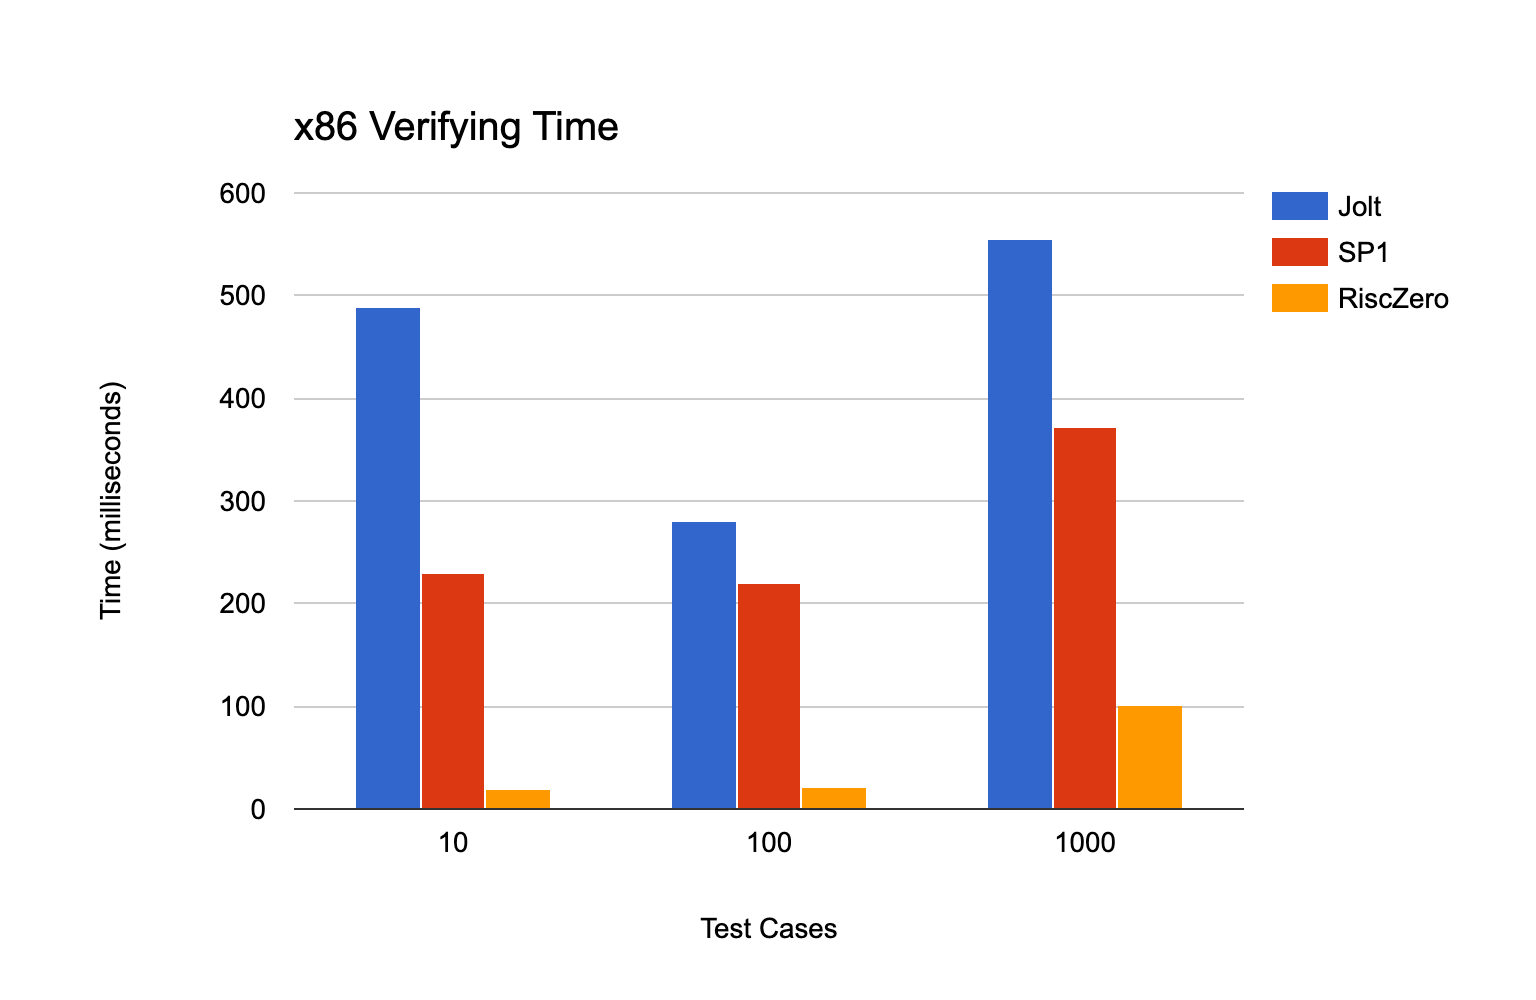
\includegraphics[width=\linewidth]{x86-Verification-Time.png}
	\end{center}
	\caption{Proof Verification Benchmark for Jolt, SP1, and RISC-0 on x86 chip}
	\label{graph:x86-verification-time}
\end{figure}


\subsection{Analysis on Benchmark Results}

Based on the benchmark results, Jolt demonstrates itself to be the most efficient zkVM in terms of proof generation across both ARM and x86 architectures. Its consistent performance highlights its suitability for real-world applications requiring rapid proof generation. While Risc0 is recognized as the first production-ready zkVM, it exhibits the poorest performance for larger test cases, particularly in proof generation. Notably, Risc0 achieves nearly twice the performance on the ARM architecture compared to x86, likely due to its architectural alignment with ARM’s RISC-based design. SP1 consistently performs between Jolt and Risc0 across both architectures, offering predictable and reliable results, with minimal variation between platforms.

Verification time does not present a significant bottleneck in real-world applications, as it is typically less critical than proof generation. Interestingly, the verification benchmarks yield almost inverse results compared to proof generation. Jolt consistently exhibits the slowest verification times across both architectures and all test cases. In contrast, Risc0 leads in verification efficiency, maintaining the fastest times regardless of architecture or test size. SP1 again performs between Jolt and Risc0, but with an anomaly in the ARM architecture at 1000 test cases, where its verification time was more than twice as slow as Jolt and nearly eight times slower than Risc0. This unexpected result may indicate a scalability issue specific to SP1 under high verification loads.

\section{Discussion}
% The discussion section focuses on the main challenges/issues you had to overcome during the project.
%
% - Outline what your approach does better than the ones you mentioned in your related work, and explain why.
% - Do the same with issues where other solutions outperform your own.
% - Are there limitations to your approach? If so, what would you recommend towards removing/mitigating them?
% - Given the experience you've gathered working on this project, are there other approaches that you feel are worth exploring?

\subsection{Contributions}
Our work differs from related work in that we focus on a holistic comparable analysis of zkVMs for real world applications. We believe our approach is more relevant than referenced papers because us focusing on zkVMs and real world applications is the most relevant for development use cases compared to other work whose results do not give you much practical insight. Additionally, compared to publicly available benchmarks, our work is unbiased and also accompanied by a qualitative architecture comparison; publicly available benchmarks do not provide such analysis.

\subsection{Limitations \& Next Steps}
Our approach had some limitations. First, we were limited by time constraints which made it difficult for us to benchmark more complicated ML models, as we would have had to implement them all from scratch for most of the VMs. We would also loved to compared more metrics such as memory usage. However, we are yet to find a publicly available benchmark that provides this comparison. Additionally, diving even deeper into the architectural design differences would have been very interesting. Finally, it would have been good for us to benchmark these VMs with and without precompiles to properly analyze the performance of the underlying design. This is an idea proposed by Justin Thaler, Professor at Georgetown University, who is a leading expert in this field. These improvements are all worth exploring in the near future.

\section{Personal Contributions}

\subsection{Siddhartha Tuladhar}

Siddhartha contributed to the serialization of the machine learning model for compatibility with Rust, the implementation of the logic required to generate zero-knowledge proofs (ZKPs) across all three zkVMs, and the development of benchmarking utilities to evaluate performance.

\subsection{Lawrence Lim}

Lawrence contributed on the ideation side in the beginning, did the cryptography research, qualitative comparisons, contributed to the ML research and led the benchmarking on the x86 and ARM HPCs.

\subsection{Brandon Gao}

\section{Conclusion}

Our paper provides a quantative and qualitative analysis on the performance of zkVMs: Jolt, SP1, and RISC-0 by generating a zero-knowledge proof of a ridge regression algorithm.  

Give a clear, short, and informative summary of all your important results. Answer the initial question(s) or respond to what you wanted to do, as stated in your introduction. It can be a short table or a list, and possibly one or two short comments or explanations.

Target a reader who may not have time to read the whole report yet, but needs the results or the conclusions immediately. This is a typical situation in real life. Some readers will read your introduction and skip to your conclusion first, and read the whole report only later (if at all).

You may also draw perspectives. What's missing? In what directions could your work be extended?



\newpage
\singlespacing
\bibliographystyle{IEEEtran}
\bibliography{references}


%------ To create Appendix with additional stuff -------%
%\newpage
%\appendix
%\section{Appendix}
%Put data files, CAD drawings, additional sketches, etc.

\end{document}

